% !TeX root = ../../main.tex
% Add the above to each chapter to make compiling the PDF easier in some editors.

\section{Generalization over users}\label{ord:ch5:sec_3_generalization_user}

% RE-1468
This benchmark study strongly benefits from having real participants applying various methods.
Valuable data is collected, which is, however, challenging to interpret.
This is because participants often have different characteristics as levels of experience, understanding of accuracy, professional background, and motivation.
As a result, the interactive method may be handled differently and the obtained data may vary with respect to various users with different characteristics. 

% Ziel = Methode zu finden mit der alles User gut klarkommen und die über verschiedene user gute Resultate in Zeit und IoU erziehlt.
However, in order to find wide application, an interactive method must work consistently with diverse users.
This section examines the generalization capabilities of the benchmark methods across different users and, therefore, is the counterpart to the previous section.
% Motivation: generalization over user -> an interactive method really performs well and reliable if it delivers good results for all possible users.




\subsection{Benchmark Participants Evaluation}\label{ord:ch5:sec3:subsec1}

In the following the performance of the methods is evaluated over the \getNumberBenchmarkParticipants participants.
In contrast to the previous evaluation, here the benchmark runs performed by the colleagues, who are working on this topic, are excluded.
This is done intentionally, in order to not distort the evaluation, since the users are explicitly evaluated here and the data obtained from most experienced users would be biased.

In order to evaluate the generalization capabilities across multiple users, first statistical key figures as the mean and standard deviation $ \sigma $ are evaluated.
The combined mean and $ \sigma $ for the participants are presented in Table \ref{tab:ch5:all_benchmark_users_varaince}.
% For IoU low std-dev, but for time vergleichsweise hoch 
It can be observed, that $ \sigma_{IoU} $ is very similar for the benchmark methods and only ranges from $ \sigma_{IoU} = 0.1187 $ for \gls{dextr} to $ \sigma_{IoU} = 0.1669 $ for watershed.
In contrast $ time $ shows a strong deviation, with $ \sigma_{time} = 15.0977 $ for \gls{dextr} the deviation is less than half as large as for polygon with $ \sigma_{time} = 39.0214 $.
The mean value is presented to put $ \sigma $ into context.
A graphical illustration of the deviation of $ IoU $ and $ time $ is already presented in the box plots from Figure \ref{fig:ch5:sec1:iou_box_plot} and \ref{fig:ch5:sec1:time_box_plot}.
Further, these results support the conclusion of Subsection \ref{ord:ch5:sec1:subsec2} and \ref{ord:ch5:sec1:subsec3}, which state that in terms of $ IoU $ the methods perform approximately equal, while $ \overline{time} $ and $ med(time) $ do differ significantly between the \gls{dl} based and classical benchmark methods.
% Calculate the variance for time and iou.
\begin{table}[h!]
	\centering
	\begin{tabular}{l|c c c c}
		\toprule 		
			 				& $ Polygon $  	& $ Watershed $ 	& $ DEXTR $ 	& $ IOG $	\\
		\midrule
		\rule{0pt}{3ex}%  EXTRA vertical height  
		$ \overline{IoU} $	& 0.8066 		& 0.8166		 	& 0.8543		& 0.8020	\\
		\rule{0pt}{3ex}%  EXTRA vertical height  
		$ \sigma_{IoU} $	& 0.1287 		& 0.1669		 	& 0.1187 		& 0.1559	\\
		\rule{0pt}{3ex}%  EXTRA vertical height  
		$ \overline{time} $	& 34.399 		& 45.076			& 14.542 		& 18.059	\\
		\rule{0pt}{3ex}%  EXTRA vertical height  
		$ \sigma_{time} $	& 39.021 		& 37.796			& 15.098 		& 17.383	\\
		\bottomrule
	\end{tabular}
	\caption[Mean and standard deviation of the benchmark methods]{
		Presentation of the mean and standard deviation $ \sigma $ for $ IoU $ and $ time $.
		It can be seen that $ \sigma_{IoU} $ stays almost constant over the benchmark methods.
		In contrast, $ \sigma_{time} $ differs between the methods.
		The mean value was given for IoU and time to better interpret $ \sigma $.
	}\label{tab:ch5:all_benchmark_users_varaince}	
\end{table}
% TODO Mir fehlt hier irgendwie eine genauere Angabe was das für Werte sind. In diesem Kapitel geht es doch um die User?     Irgendwo (vllt auch als Formel) sollte gezeigt werden, dass hier ein Mittel über die User-weisen Mittel (mean_mean_IoU_per_user_per_method) gebildet wird.     Genauso ist das wohl die mittlere Varianz (gemittelt über die User), oder?


To get even deeper insights about the generalization across different users, in Figure \ref{fig:ch5:sec3:all_benchmark} box plots for $ IoU $ and $ time $ are shown for all participants individually.
Here, no statistical tests for equality within the methods were performed, because the visualization already indicates that there are strong deviations between the user for each method.
The variations between the individual users are present in all methods and most likely due to the varying characteristics of the users as introduced in the beginning of this section.
% \eg different experience levels, how , and how well a user got along with the method.

However, it can be stated that for $ IoU $ \gls{dextr} has the smallest deviation and is the most constant method over all participants, while the other methods still perform similar.

% Box plot of all BenchmarkParticipants (not experienced user aka me)
\begin{figure} 
	\centering
	\begin{subfigure}[t]{1.0\textwidth}
		\centering
		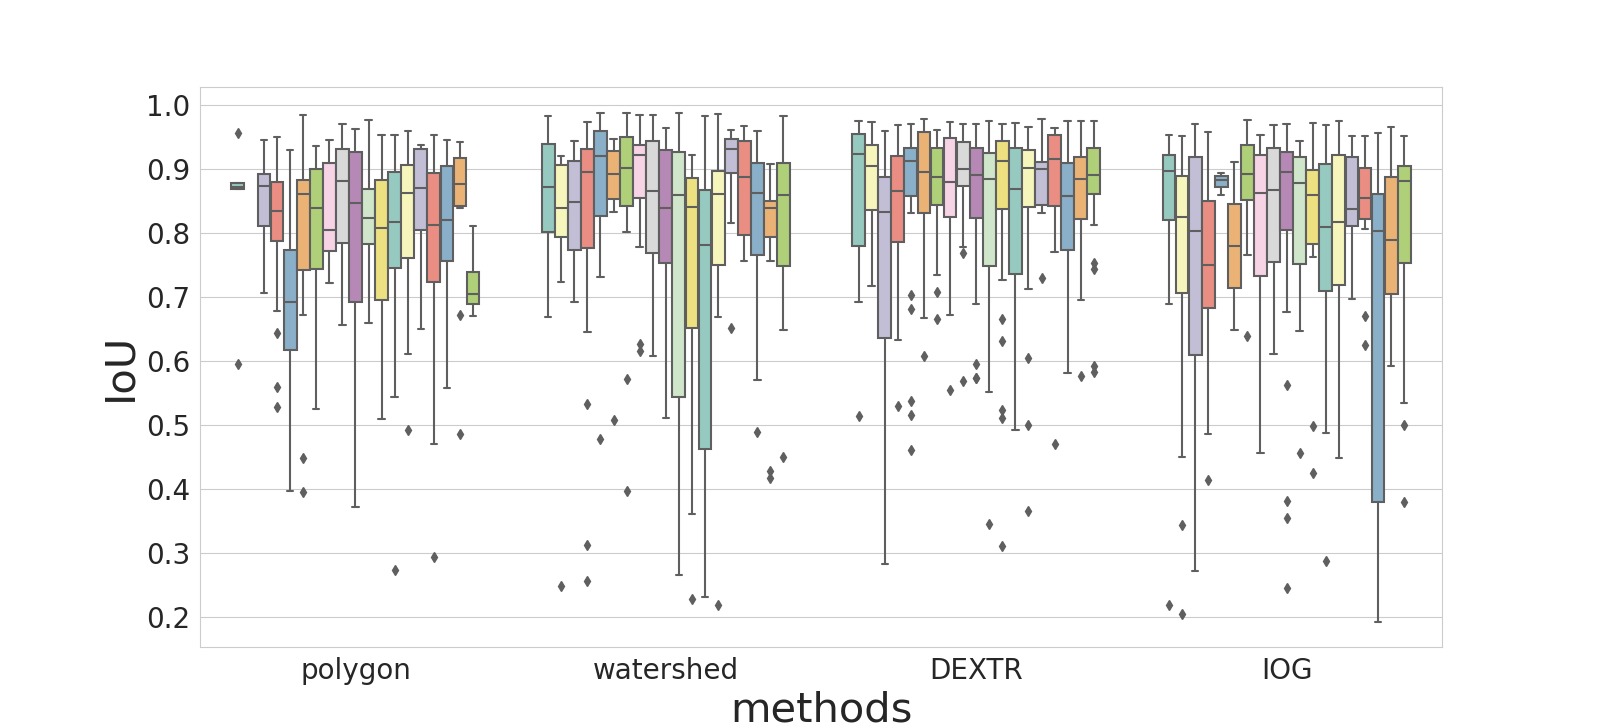
\includegraphics[width=\textwidth]{figures/chap53_all_users_iou.png}
		\caption{
			The \gls{dextr} delivers mostly constant $ IoU $ values with some outliers, while the other methods are mostly characterized by irregularities.
		}\label{fig:ch5:sec3:all_benchmark_iou}
	\end{subfigure}
	\\
	\begin{subfigure}[t]{1.0\textwidth}
		\centering
		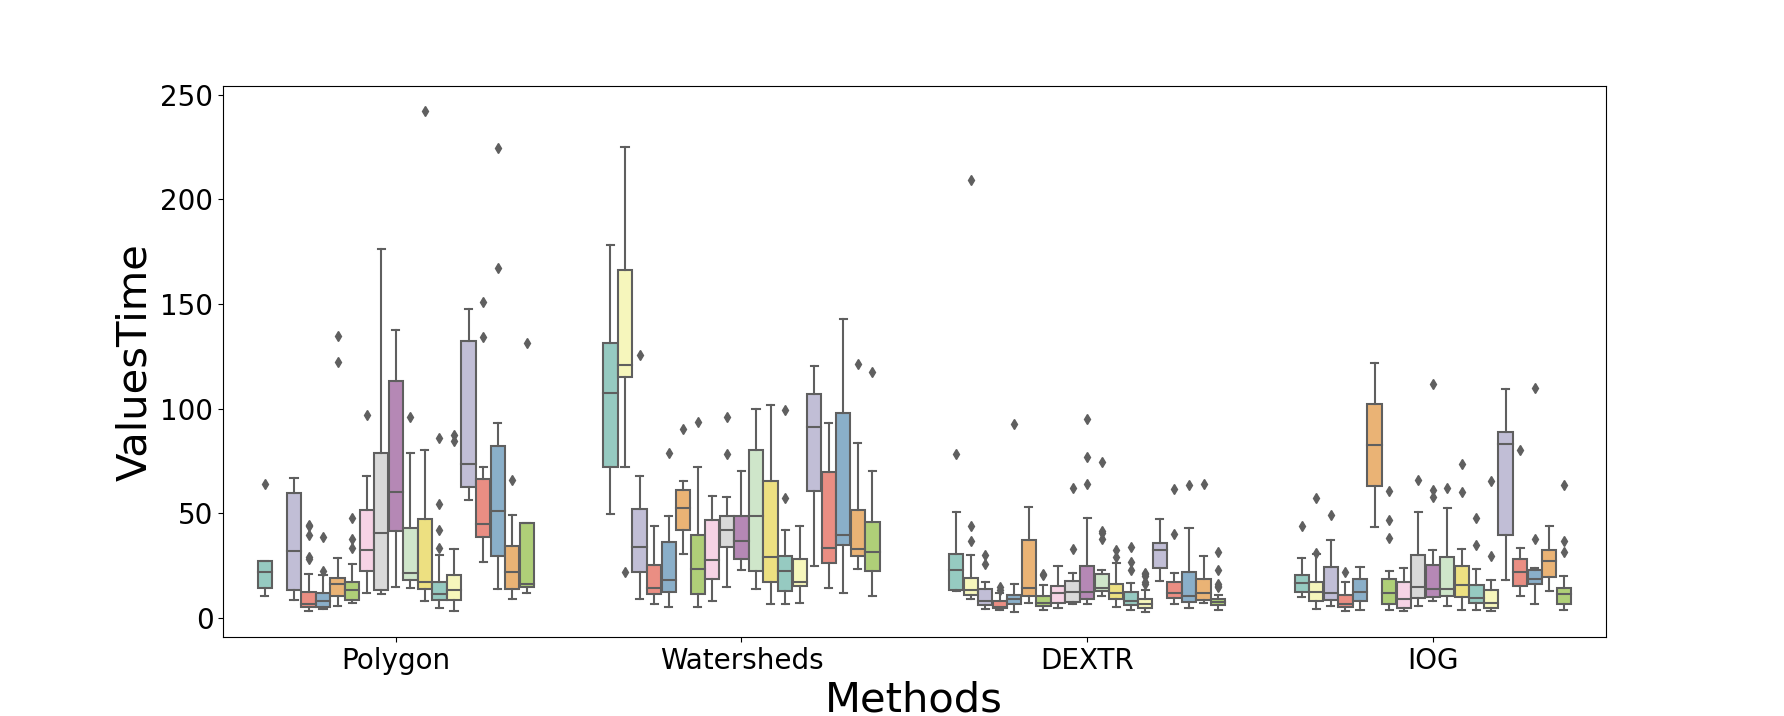
\includegraphics[width=\textwidth]{figures/chap53_all_users_time.png}
		\caption{
			For $ time $ the \gls{dextr} method convinces with a mostly constant performance, while the \gls{iog} method has two users who are the exception to the consistency.
			In contrast for the polygon and watershed method consistency over various user is not given.			
		} \label{fig:ch5:sec3:all_benchmark_time}
	\end{subfigure}
	\caption[Box plots of benchmark participants on $ IoU $ and $ time$.]{		
		The box plots of $ IoU $ and $ time $ over the \getNumberBenchmarkParticipants benchmark participants.
		The single box plots indicate how the methods performed over the single users, the order of the users is the same for both figures. 
		Large differences between the box plots within a method indicate poor generalization capabilities and vice versa.
	}\label{fig:ch5:sec3:all_benchmark}
\end{figure}

In terms of $ time $ the \gls{dl} based methods show less variance over the users than the classical methods.
The \gls{dextr} method performs best, while the \gls{iog} method has two bigger outliers.
The difference between \gls{dl} based and classical methods is partly caused by the design of the methods, which guides the user more or less.
On the one side, the polygon and watershed method do little to guide the user,
but give the user a lot of freedom when performing the label task.
This room for interpretation is used differently by the users, which leads to different label times and, therefore, higher variance.
On the other side, the \gls{dextr} and \gls{iog} method provide strong guidance by defining the amount of clicks required for an initial prediction.
Although the application of refinement is still possible, this prevents users from spending too much time on an initial prediction.
This strong guidance of the user while applying the method leads to a more constant annotation time and thereby a lower variance in $ time $.
% polygon and watershed are more freely

In conclusion, for $IoU$ the \gls{dextr} method generalizes best over multiple users, while the other models do no achieve a constant performance over various users.
For $ time $ it is observed, that methods with strong guidance as \gls{dextr} and \gls{iog} are more constant in $ time $, than the polygon and watershed method, that are designed more open and, therefore, allow higher variance.


\subsection{Two Experienced Users} \label{ord:ch5:sec3:subsec2_cmo_afe}

Normally, the participants have labeled only a part of the benchmark images. 
In the following, eight benchmark runs are evaluated where all benchmark images were labeled by two users who have more experience working on this topic.
Although only two different users are compared with each other, the significance is given, since all images of the benchmark were labeled.
However, it must be mentioned that the experience level of both users is not the same, because $ \textnormal{\textit{User 2}} $ is more trained than $ \textnormal{\textit{User 1}} $.

% No significant difference in the IoU between the two user could be detected -> generalize well over various users (few user, large data)
For the $ IoU $, the box plots in Figure \ref{fig:ch5:sec3:cmo_afe_iou} indicate, that the $ IoU $ is more or less equal fors $ \textnormal{\textit{User 1}} $ and $ \textnormal{\textit{User 2}} $ for the four benchmark methods.
The equality of the obtained values from both users are statistically confirmed by the Kruskal-Wallis test, the details of the tests are presented in Table \ref{tab:appendix:afe_cmo_kruskal_wallis_iou}.

An equivalent analysis was performed for $ time $, as presented in Figure \ref{fig:ch5:sec3:cmo_afe_time}.
Interestingly, here the annotation time between $ \textnormal{\textit{User 1}} $ and $ \textnormal{\textit{User 2}} $ differs strongly for polygon and watershed, while the annotation time is very similar for \gls{dextr} and \gls{iog}.
The statistical relevance of this observation is again confirmed by the Kruskal-Wallis test, presented in detail in Table \ref{tab:appendix:afe_cmo_kruskal_wallis_time}.

\begin{figure} [h!]
 	\centering
 	\begin{subfigure}[t]{0.45\textwidth}
 		\centering
 		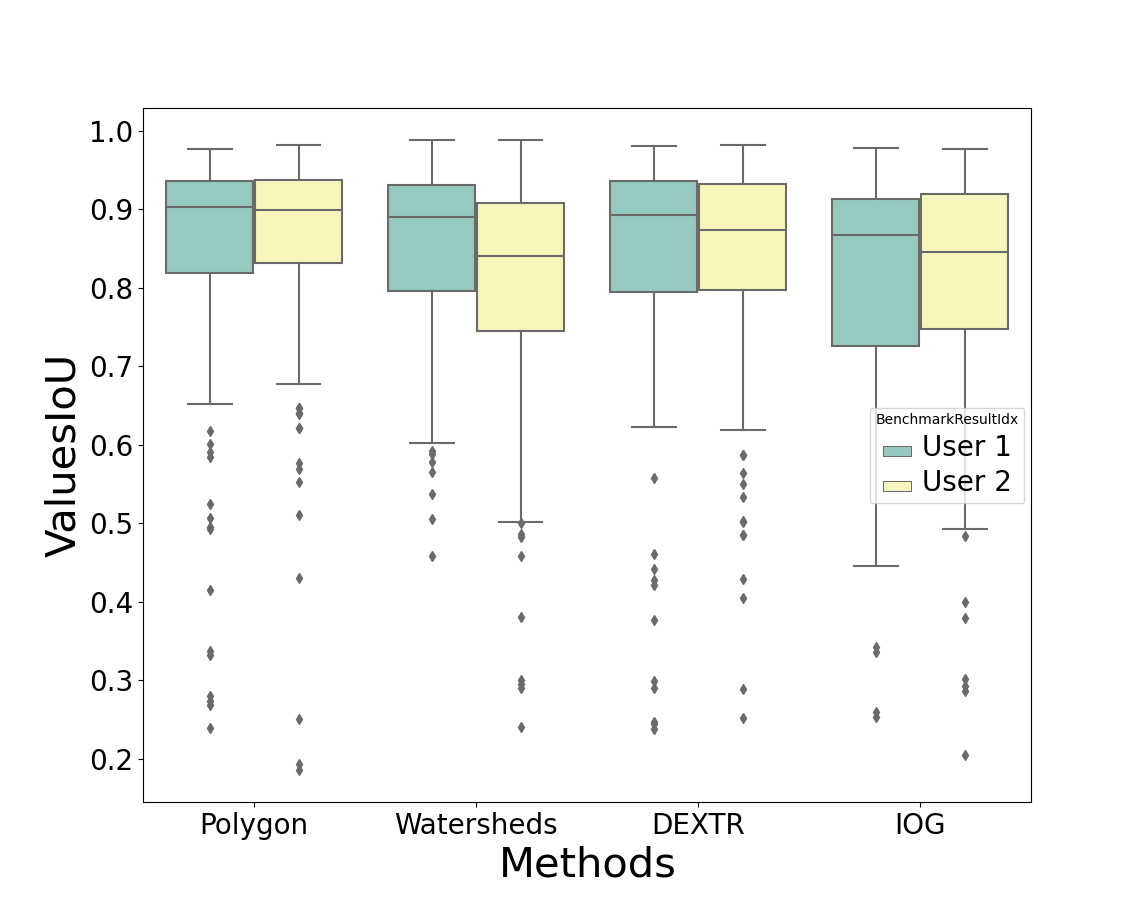
\includegraphics[width=\textwidth]{figures/chap53_afe_cmo_iou.png}
 		\caption{
 			Box plots of the $ IoU $ for the four benchmark methods of $ \textnormal{\textit{User 1}} $ and $ \textnormal{\textit{User 2}} $.
 			The visualization does not indicate any significant difference in $ IoU $.
 		} \label{fig:ch5:sec3:cmo_afe_iou}
 	\end{subfigure}
 	\hfill
 	\begin{subfigure}[t]{0.45\textwidth}
 		\centering
 		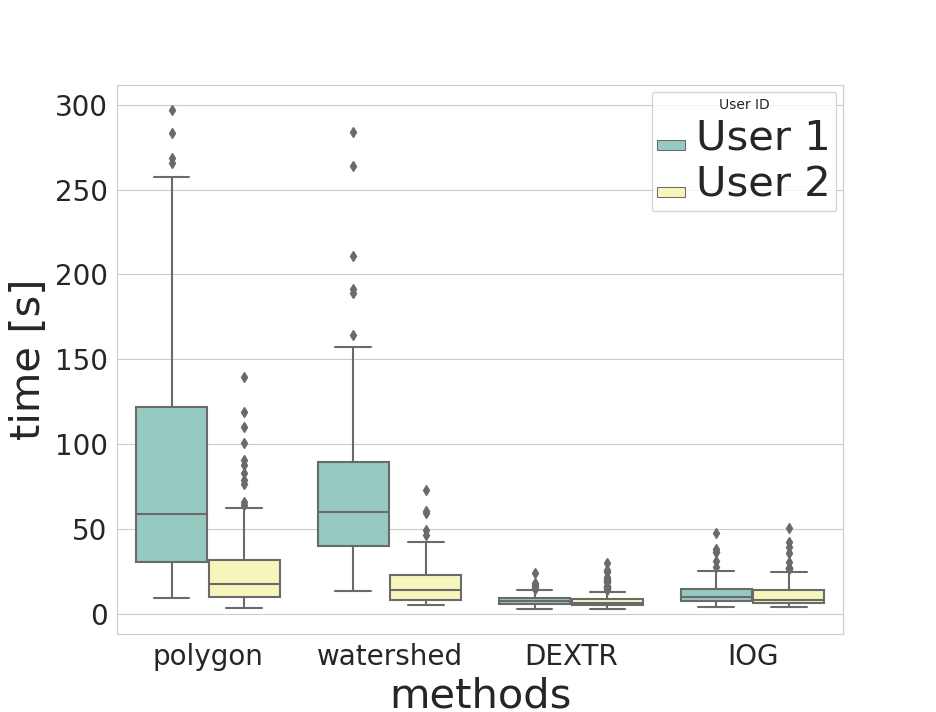
\includegraphics[width=\textwidth]{figures/chap53_afe_cmo_time.png}
 		\caption{
 			Box plots of the $ time $ for the four benchmark methods of $ \textnormal{\textit{User 1}} $ and $ \textnormal{\textit{User 2}} $.
 			A significant difference in $ time $ for the polygon and watershed is shown, while the \gls{dextr} and \gls{iog} methods perform similar.
 		}\label{fig:ch5:sec3:cmo_afe_time}
 	\end{subfigure}
 	\caption[Box plots of two experienced user on $ IoU $ and $ time$.]{		
 		These two figures show the comparison of the two users over the benchmark methods based on $ IoU $ and $ time $.
 		The hypothesis based on the graphical visualizations are statistically supported by the Kruskal-Wallis test as presented in detail in Table \ref{tab:appendix:afe_cmo_kruskal_wallis_iou} and \ref{tab:appendix:afe_cmo_kruskal_wallis_time}.
 	}\label{fig:ch5:sec3:cmo_afe}
\end{figure}

% User 2 more experienced that User 1
This large difference for Polygon and Watershed was not expected, but it emphasizes again how large the variance can be between different users who achieve the same performance.
This difference may be partly caused by the different level of experience of the two users.
Anyway, it is not surprising that this occurs for the classical methods, that are more freely interpretable and, therefore, leave the user a more open application.
Rather this supports the conclusion of the previous subsection, that methods with stronger guidance perform more consistent in the annotation time.


\subsection{Simulations With Different Click Patterns}\label{ord:ch5:sec3:subsec3}
% RE-1468

% Simulations are easily scalable, faster and cheaper than the acquisition of manual clicks from real users.
% Second, in a simulation no variance occurs between the set clicks of various users, if the.
% Third, simulations have the possibility to effortless create various click patterns, that \eg vary the set click by a random offset, in order to simulate a various types of user behavior.
%On the other hand, simulations are only capable to replicate the user's behavior to a certain extent.
% Further, the involvement of human users is especially important for methods, which performance depends on user interactions.


In order to gain deeper insights on the functionality of the \gls{dextr} and \gls{iog} method the simulation setup is modified.
% Motivation - Nachahmung von unterschiedlichen Usertypen durch unterschiedliche Genauigkeit bei der Klick-Simulation.
The altered simulation setup uses different levels of accuracy, to simulate more realistic user clicks.
% Simulation of with different permutation / deviation / - simulation of different user

The level of accuracy is defined by a deviation of maximal $ n_{deviation} $ \Unit{px}.
In the range $ \left[-n_{deviation}, \dots, 0, \dots, n_{deviation} \right] $ two values are randomly selected and added to the ideal row and column.
This random factor was added, to simulate the varying accuracy of single user clicks.
The smaller $ n_{deviation} $, the more accurate are the simulated clicks.
In the simulation first the ideal click position is calculated and further the random deviation is added.
This procedure is applied to the extreme points of the \gls{dextr} method and to the foreground and background clicks of the \gls{iog} method.
\begin{table}[h!]
	\centering	
	\resizebox{\textwidth}{!}{
	\begin{tabular}{l l|c c c c c c c}
		\toprule
				&						& \multicolumn{7}{c}{mIoU} \\
				& {$ n_{deviation} $} 	& 0	\Unit{px}	& 5	\Unit{px}	& 10 \Unit{px}	& 15 \Unit{px}	& 20 \Unit{px}	& 25 \Unit{px}	& 30 \Unit{px}	\\
		\midrule
		DEXTR 	& PASCAL (VP \cmark)	& 0.9103	& 0.8323	& 0.7626	& 0.7032 	& 0.6479	& 0.6047	& 0.5626		\\
				& PASCAL (VP \xmark)	& 0.7807	& 0.7523	& 0.7019	& 0.6543 	& 0.6085	& 0.5695	& 0.5317		\\
				& Benchmark				& 0.8414	& 0.7743	& 0.6887	& 0.6240 	& 0.5579	& 0.5027	& 0.4892		\\
		\midrule
		IOG 	& PASCAL (VP \cmark)	& 0.9267	& 0.8846	& 0.8092	& 0.7352 	& 0.6578	& 0.5953 	& 0.5457		\\
				& PASCAL (VP \xmark)	& 0.8081	& 0.7720	& 0.7099	& 0.6476 	& 0.5979	& 0.5337	& 0.4873		\\
				& Benchmark				& 0.8219	& 0.7865	& 0.7173	& 0.6027 	& 0.5268	& 0.4493 	& 0.4058		\\
		\bottomrule
	\end{tabular}}
	\caption[Simulations with different click patterns]{
		Simulations of the \gls{dextr} and \gls{iog} method with user clicks, that are simulated with varying degrees of accuracy.
		The parameter $ n_{deviation} $ states the maximal possible deviation from the optimal point, in order to mimic different types of users.
		As expected, the performance decreases with increasing deviation in the simulated user clicks.
	}\label{tab:ch5:simulation_various_click_patterns}
\end{table}

The performance constantly decreases with higher $ n_{deviation} $, as demonstrated in Table \ref{tab:ch5:simulation_various_click_patterns}. 
Even a comparable small deviation of maximal 5 \Unit{px} leads a notable drop in performance \eg from $ mIoU = 0.9103 $ to 0.8323 for \gls{iog} on the PASCAL \gls{voc} dataset with the application of \gls{vp}.
This factor needs to be taken into account, if these methods are applied by real users.




